\documentclass{article}
\usepackage{enumerate}
\usepackage{amsmath}
\usepackage{amssymb}
\usepackage{graphicx}
\usepackage{subfigure}
\usepackage{geometry}
\usepackage{color}
\usepackage{bm}
\usepackage{indentfirst}

\begin{document}

\vspace*{0.25cm}

\hrulefill

\thispagestyle{empty}

\begin{center}
\begin{large}
\sc{UM--SJTU Joint Institute \vspace{0.3em} \\ Physics Laboratory \\(Vp141)}
\end{large}

\hrulefill

\vspace*{5cm}
\begin{Large}
\sc{{Laboratory Report}}
\end{Large}

\vspace{2em}

\begin{large}
\sc{{Exercise 4
\vspace{0.5em}

Measurement of the Speed of Sound
}}
\end{large}
\end{center}


\vfill

\begin{table}[h!]
\flushleft
\begin{tabular}{lll}
Name: Yihao Liu \hspace*{2em}&
ID: 515370910207\hspace*{2em}\\
Name: Yichen Hu \hspace*{2em}&
ID: 515370910044\hspace*{2em}
& Group: 7\\


\\

Date: 28 June 2016 

\end{tabular}
\end{table}

\hfill
\begin{tiny}
[rev. 1.0]
\end{tiny}
\newpage

\section{Introduction}

The objective of this exercise to study several methods of measuring the speed of
sound in air: the resonance method, the phase comparison method, and the time difference
method. In addition, you will get familiar with the successive difference method in
measurement data processing.
\\

\subsection{Basic Quantitative Characteristics of Sound Waves}

Sound is a mechanical wave that propagates through a compressible medium. It is a
longitudinal wave because the direction of vibrations of the medium (here, change in the
density or the pressure) is the same as the direction of propagation. The frequency of
sound perceptible to a human ear ranges from about 20 Hz to 20 000 Hz. Sound with the
frequency higher than 20 000 Hz is called ultrasound. In this experiment an ultrasonic
wave is chosen as the signal source, because its wavelength is short enough to measure
the speed of sound precisely.
\\

The phase speed $v$, the frequency $f$ and the length $\lambda$ of a wave are related by the
formula
\begin{equation}\label{eq-1}
v=\lambda f
\end{equation}

For motion with constant speed $v$ along a straight line, we have
\begin{equation}\label{eq-2}
v=\frac{L}{t}
\end{equation}

where $L$ is the distance traveled over time $t$. Hence, if the distance and the time a
wavefront travels is known, the phase speed may be found.

\section{Experimental setup}

The experimental setup consists of a signal source, two piezoelectric transducers $S_1$
and $S_2$, and oscilloscope arranged as shown in Figure \ref{fig-1}.

\begin{figure}[!h]
	\centering
	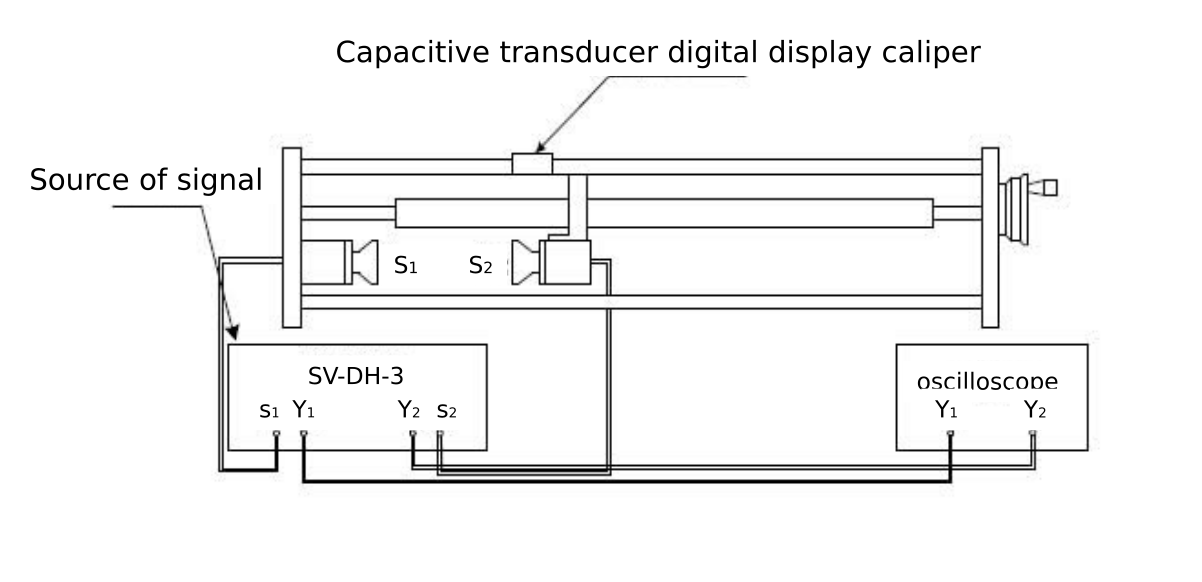
\includegraphics[width=13cm]{fig-1.png}
	\caption{Experimental setup.
	\label{fig-1}}
\end{figure}

\subsection{Resonance Method}

The elements $S_1$ and $S_2$ are the wave source and the receiver (also reflector), respectively, placed a distance $L$ from each other. If they are arranged parallel to each other,
the sound wave is reflected. If

\begin{equation}\label{eq-3}
L=n\frac{\lambda}{2}
\end{equation}

where $n$ = 1, 2, . . ., i.e. the distance is a multiple of half-wavelength, standing waves will
form, and maximum output power will be observed in the oscillograph (Figure 2). The
distance between two successive maxima ($L_{i+1}-L_i$ ) is always $\lambda/2$. After the position
corresponding to each maximum is measured, it is easy to find the wavelength and then
the speed of sound by using Eq. (\ref{eq-1}). The frequency $f$ is displayed directly on the signal
generator.

\subsection{Phase-comparison method}
If the phase of the wave at two points on the wave propagation direction is equal, then
the distance between these points $L$ has to be a multiple of the wavelength, $i.e.$

$$ L=n\lambda $$

where $n$ = 1, 2, . . .. The experimental setup for the phase comparison method is the same
as in the previous method (Figure \ref{fig-1}). Lissajous figures are used to identify the values of
$L$. Lissajous figures (or Lissajous curves) are trajectories of a particle that moves in a
plane so that i.e. it moves in a harmonic motion independently along two perpendicular
directions (for example the axes x and y of a Cartesian coordinate system), so that $r(t)=(Ax\cos(\omega x t+\varphi x),Ay\cos(\omega yt+\varphi y))$. When the two superimposed harmonic motions have
identical frequency $\omega x = \omega y$ and phase difference $|\varphi x − \varphi y |$ = nπ, where $n$ = 0, 1, 2, . . .,
the Lissajous figure will show as a straight line. For other values of the phase difference
the figures will have an elliptical shape.

\subsection{Time-difference method}
When an ultrasonic pulse signal emitted by $S_1$ arrives at $S_2$ , it is received and returned
back to the processor. By contrasting the original signal with the received one, one can
measure the time needed for the sound to travel from $S_1$ to $S_2$ over a distance of $L$. When
the values of $L$ and $t$ are known, the phase speed of sound can be found from Eq. (\ref{eq-2}).

\subsection{Successive Difference Method}
The successive difference method is an effective method to increase the accuracy of
the average value calculated from a series of measurement data. In this experiment, the
usual method of calculating the average value, illustrated by the formula

\begin{equation}\label{eq-4}
\frac{\bar{\lambda}}{2}=\frac{[(L_1-L_0)+(L_2-L_1)+\cdots+(L_n-L_{n-1})]}{n}=\frac{L_n-L_0}{n}
\end{equation}

will be modified, because as Eq. (\ref{eq-4}) shows, the average value of the wavelength is determined only by the first and the last value, $L_0$ and $L_n$ .
\\

A modification of the formula by rearranging terms as

\begin{equation}\label{eq-5}
n\frac{\bar{\lambda}}{2}=\frac{\sum_{i=1}^n(L_{n+i}-L_i)}{n}
\end{equation}

produces more accurate results, as each value contributes to the final result.

\begin{figure}[!h]
	\centering
	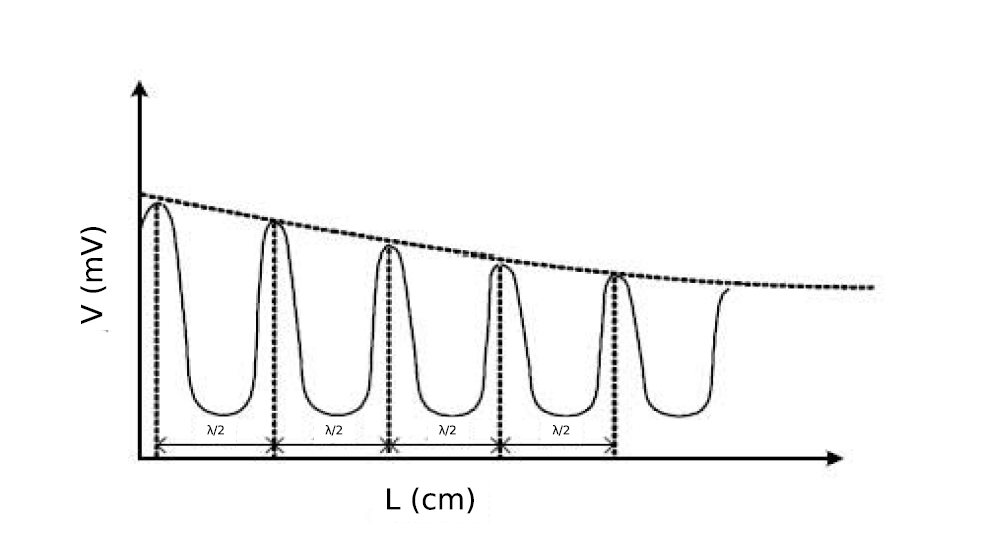
\includegraphics[width=13cm]{fig-2.png}
	\caption{Relationship between the signal voltage and the distance between the transducers.
	\label{fig-2}}
\end{figure}

\section{Measurement}

\subsection{Resonance Method}

\begin{enumerate}
\item
Set the initial distance between $S_1$ and $S_2$ at about 1 cm.
\item
Turn on the signal source and the oscilloscope. Then set the following options on
the panel of the signal source
\begin{enumerate}[(1)]
	\item
	Choose Continuous wave for Method.
	\item
	Choose Air for Medium.
	\item
	Adjust Signal Strength until a 10 V peak voltage is observed on the oscilloscope.
	\item
	Adjust Signal Frequency between 34.5 and 37.5 kHz until the peak-to-peak voltage reaches its maximum. Record the frequency.
\end{enumerate}
\item
Increase $L$ gradually by moving $S_2$ , and observe the output voltage of $S_2$ on the
oscilloscope. Record the position of $S_2$ as $L_2$ when the output voltage reaches an
maximum.
\item
Repeat step 3 to record 20 values of $L_2$ and calculate $v$.
\end{enumerate}

\subsection{Phase-comparison Method}
\begin{enumerate}
\item
Use Lissajous figures to observe the phase difference between the transmitted and
the received signals. Move $S_2$ and record the position when the Lissajous figure
becomes a straight line with the same slope.
\item
Repeat step 1 to collect 12 sets of data. Use the successive difference method to
process the data and calculate $v$.
\end{enumerate}

\subsection{Time-difference Method}
Since the pulse wave causes damped oscillations at the receiver, there will be significant
interference if $S_1$ and $S_2$ resonate. The resonance can be observed on the oscilloscope.
\begin{enumerate}
\item
Choose Pulse Wave for Method and Air for Medium on the panel of the signal
source.
\item
Adjust the frequency to 25 Hz and the width to 500 μs.
\item
Record the distance $L_1$ and the time $t_1$ .
\item
Move $S_2$ to another position and repeat step 3. Record $L_i$ and $t_i$ , $i$ = 2, 3, 4, . . .
\item
Repeat step 4 to collect 12 pairs of $L_i$ and $t_i$ . Plot the $L_i = L_i (t_i)$ graph and use
computer software to find a linear fit to the data. The slope of the line is the speed $v$.
\end{enumerate}

\subsection{Time-difference Method in a Liquid}

\begin{enumerate}
\item
Change the medium to water.
\item
Adjust the frequency to 100 Hz and the width to 500 μs.
\item
Use the cursor function of the oscilloscope to measure the time and the distance
between the the starting points of neighboring periods. Record 12 pairs of data and
calculate $v_{water}$ .
\end{enumerate}

\section{Results}

The frequency of the sound wave was measured as
$$f=35.43\pm0.01\,\rm{kHz}$$

The temperature was measured as
$$T=28\pm1\,\rm{^\circ C}$$

\subsection{Resonance Method}

The measurement of length $L$ was shown in Table \ref{tab-1}.

\begin{table}[!h]
\begin{center}
\begin{tabular}{|c|c||c|c||c|c|}
\hline
\multicolumn{2}{|c||}{$L_i$ [mm] $\pm$ 0.01 [mm]} &
\multicolumn{2}{|c||}{$L_i$ [mm] $\pm$ 0.01 [mm]} &
\multicolumn{2}{|c|}{$L_{10+i}-L_i$ [mm]} \\
\hline
1 & 14.66 & 11 & 64.60 & 1 & 49.94 \\
2 & 19.56 & 12 & 69.63 & 2 & 50.07 \\
3 & 24.69 & 13 & 74.47 & 3 & 49.78 \\
4 & 29.73 & 14 & 79.56 & 4 & 49.83 \\
5 & 34.73 & 15 & 84.52 & 5 & 49.79 \\
6 & 39.63 & 16 & 89.43 & 6 & 49.80 \\
7 & 44.74 & 17 & 94.43 & 7 & 49.69 \\
8 & 49.63 & 18 & 99.34 & 8 & 49.71 \\
9 & 54.69 & 19 & 104.37& 9 & 49.68 \\
10& 59.65 & 20 & 109.22& 10& 49.57 \\
\hline
\end{tabular}
\caption{Data table for the resonance method.}
\label{tab-1}
\end{center}
\end{table}

$$v=\bar{\lambda}f=\frac{2f\sum_{i=1}^{10}(L_{10+i}-L_i)}{n^2}=352.78\pm 2\,\rm{m/s}$$

\subsection{Phase-comparison Method}

The measurement of length $L$ was shown in Table \ref{tab-2}.

\begin{table}[!h]
\begin{center}
\begin{tabular}{|c|c||c|c||c|c|}
\hline
\multicolumn{2}{|c||}{$L_i$ [mm] $\pm$ 0.01 [mm]} &
\multicolumn{2}{|c||}{$L_i$ [mm] $\pm$ 0.01 [mm]} &
\multicolumn{2}{|c|}{$L_{6+i}-L_i$ [mm]} \\
\hline
1 & 14.53 & 11 & 74.45 & 1 & 59.92 \\
2 & 24.70 & 12 & 84.39 & 2 & 59.96 \\
3 & 34.49 & 13 & 94.33 & 3 & 59.84 \\
4 & 44.66 & 14 & 104.23& 4 & 59.57 \\
5 & 54.44 & 15 & 114.16& 5 & 59.72 \\
6 & 64.54 & 16 & 124.09& 6 & 59.55 \\
\hline
\end{tabular}
\caption{Data table for the phase comparison method.}
\label{tab-2}
\end{center}
\end{table}

$$v=\bar{\lambda}f=\frac{f\sum_{i=1}^{6}(L_{6+i}-L_i)}{n^2}=352.56\pm 2\,\rm{m/s}$$

\newpage

\subsection{Time-difference Method}

The measurement of time $t$ and length $L$ was shown in Table \ref{tab-3}.

\begin{table}[!h]
\begin{center}
\begin{tabular}{|c|c|c|}
\hline
& $t_i$ [$\mu$s] $\pm$ 0.5 [$\mu$s] & $L_i$ [mm] $\pm$ 0.01 [mm] \\
\hline
1 & 23.5 & 10.00 \\
2 & 51.5 & 20.00 \\
3 & 80.0 & 30.00 \\
4 & 107.5& 40.00 \\
5 & 134.5& 50.00 \\
6 & 163.0& 60.00 \\
7 & 192.5& 70.00 \\
8 & 220.5& 80.00 \\
9 & 249.0& 90.00 \\
10& 276.5& 100.00 \\
11& 306.0& 110.00 \\
12& 334.5& 120.00 \\
\hline
\end{tabular}
\caption{Data table for the time difference method.}
\label{tab-3}
\end{center}
\end{table}

\begin{figure}[!h]
	\centering
	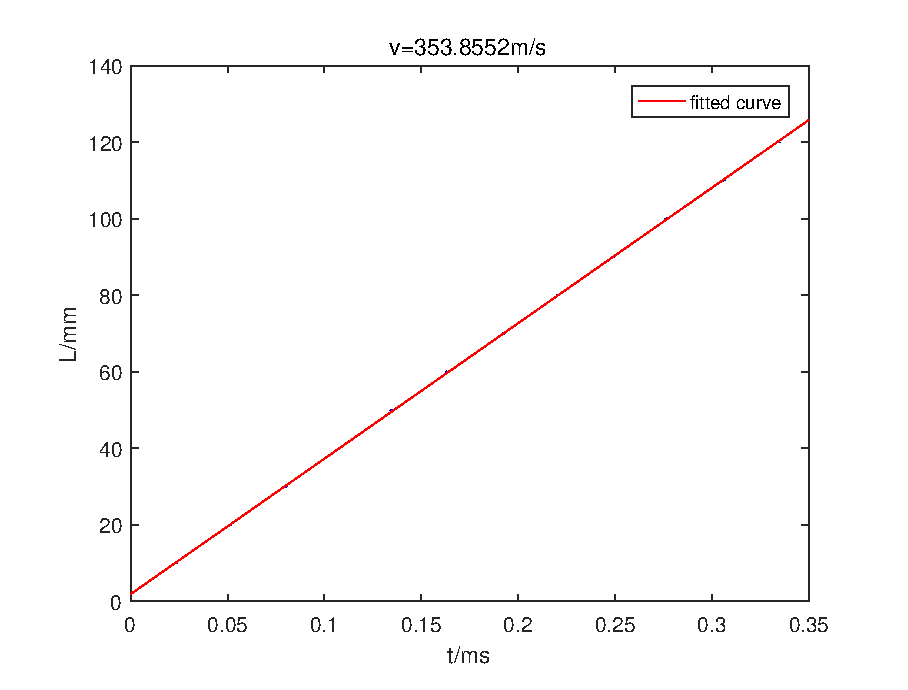
\includegraphics[width=10cm]{fig-3.eps}
	\caption{Relation ship between $L_i$ and $t_i$.
	\label{fig-3}}
\end{figure}

$$v=353.86\pm0.3\,\rm{m/s}$$

\newpage

\subsection{Time-difference Method in a Liquid}


The measurement of time $t$ and length $L$ was shown in Table \ref{tab-4}.

\begin{table}[!h]
\begin{center}
\begin{tabular}{|c|c|c|}
\hline
& $t_i$ [$\mu$s] $\pm$ 0.2 [$\mu$s] & $L_i$ [mm] $\pm$ 0.01 [mm] \\
\hline
1 & 32.2 & 10.00 \\
2 & 37.6 & 20.00 \\
3 & 43.6 & 30.00 \\
4 & 49.4 & 40.00 \\
5 & 55.4 & 50.00 \\
6 & 62.6 & 60.00 \\
7 & 69.0 & 70.00 \\
8 & 75.6 & 80.00 \\
9 & 82.0 & 90.00 \\
10& 89.0 & 100.00 \\
11& 95.6 & 110.00 \\
12& 102.0& 120.00 \\
\hline
\end{tabular}
\caption{Data table for the time difference method in liquid.}
\label{tab-4}
\end{center}
\end{table}

\begin{figure}[!h]
	\centering
	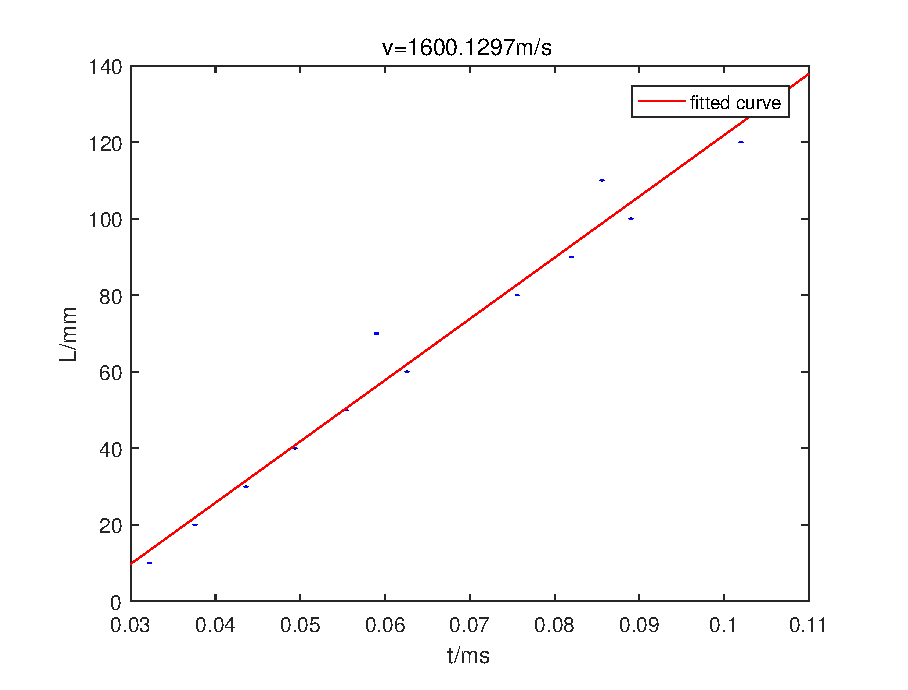
\includegraphics[width=10cm]{fig-4.eps}
	\caption{Relation ship between $L_i$ and $t_i$ in liquid.
	\label{fig-4}}
\end{figure}

$$v_{water}=1600.13\pm6\,\rm{m/s}$$


\newpage

\section{Measurement uncertainty analysis}

\subsection{Resonance Method}
For a single measurement of $\Delta L=L_{n+i}-L_i$, its uncertainty (of
type B) is $\Delta_{\Delta LB}=\Delta_{dev}=0.01mm$. In the experiment, $\overline{\Delta L}$ is found by 
taking the average of 10 measurements. In order to estimate type-A uncertainty of the time, the standard deviation of the average value is calculated as
$$S_{\Delta L}=\sqrt{\frac{1}{n(n-1)}\sum_{i=1}^n(\Delta L-\overline{\Delta L}{})^2}$$

Using the data from Table.\ref{tab-1} one obtains $S_{\Delta L}=0.141mm$. Taking into account that $t_{0.95}=2.26$ for $n=10$, the Type-A uncertainty is estimated as $\Delta_{\Delta L A}=2.26\cdot0.141=0.32mm$

Hence the combined uncertainty
$$u_{\Delta L}=\sqrt{\Delta^2_{\Delta L A}+\Delta^2_{\Delta L B}}=\sqrt{0.32^2+0.01^2}=0.32mm$$

$v$ can be calculated by the equation $v=\frac{2f\Delta L}{n}$. Therefore its uncertainty $u_{v}$ is found by applying the uncertainty propagation formula

\begin{align*}
u_v&=\sqrt{\left(\frac{\partial v}{\partial f}\right)^2u_f^2+\left(\frac{\partial v}{\partial \Delta L}\right)^2u_{\Delta L}^2}\\
&=\sqrt{\left(\frac{2\Delta L}{n}\right)^2u_f^2+\left(\frac{2f}{n}\right)^2u_{\Delta L}^2}\\
&=2.27\,\rm{m/s}
\end{align*}

Hence the density of the balls found from the measurement of the fixed mass and diameter is
$$v=352.78\pm2\,\rm{m/s}$$

with relative uncertainty 0.57\%

\subsection{Phase-comparison Method}

For a single measurement of $\Delta L=L_{n+i}-L_i$, its uncertainty (of
type B) is $\Delta_{\Delta LB}=\Delta_{dev}=0.01mm$. In the experiment, $\overline{\Delta L}$ is found by 
taking the average of 10 measurements. In order to estimate type-A uncertainty of the time, the standard deviation of the average value is calculated as
$$S_{\Delta L}=\sqrt{\frac{1}{n(n-1)}\sum_{i=1}^n(\Delta L-\overline{\Delta L}{})^2}$$

Using the data from Table.\ref{tab-1} one obtains $S_{\Delta L}=0.15mm$. Taking into account that $t_{0.95}=2.57$ for $n=6$, the Type-A uncertainty is estimated as $\Delta_{\Delta L A}=2.57\cdot0.15=0.39mm$

Hence the combined uncertainty
$$u_{\Delta L}=\sqrt{\Delta^2_{\Delta L A}+\Delta^2_{\Delta L B}}=\sqrt{0.39^2+0.01^2}=0.39mm$$

$v$ can be calculated by the equation $v=\frac{f\Delta L}{n}$. Therefore its uncertainty $u_{v}$ is found by applying the uncertainty propagation formula

\begin{align*}
u_v&=\sqrt{\left(\frac{\partial v}{\partial f}\right)^2u_f^2+\left(\frac{\partial v}{\partial \Delta L}\right)^2u_{\Delta L}^2}\\
&=\sqrt{\left(\frac{\Delta L}{n}\right)^2u_f^2+\left(\frac{f}{n}\right)^2u_{\Delta L}^2}\\
&=2.31\,\rm{m/s}
\end{align*}

Hence the density of the balls found from the measurement of the fixed mass and diameter is
$$v=352.56\pm2\,\rm{m/s}$$

with relative uncertainty 0.57\%

\subsection{Time-difference Method}
According to MATLAB,

$$v=353.86\pm0.3\,\rm{m/s}$$

with relative uncertainty 0.08\%

$$v_{water}=1600.13\pm6\,\rm{m/s}$$

with relative uncertainty 0.46\%

\section{Conclusion}

In this experiment, we measured the speed of sound in three different methods.
\\

According to the data, we can conclude that the speed of sound in the air is about 350 m/s and the speed of sound in a certain liquid is 1600 m/s, which is similar to data from the Internet.
\\

The uncertainty of the data is quite small, which suggests that the experiment is accurate.

\section{Reference}
\begin{enumerate}[(a)]
	\item
	Qin Tian, Cao Jianjun, Yi Hankun, Mateusz Krzyzosiak, VP141 Exercise 4, Measurement of the Speed of Sound, based on materials provided by the Department of Physics, Shanghai Jiaotong University.
\end{enumerate}


\end{document}